\documentclass[times, doublespace]{anzsauth}
\usepackage[]{times}
\usepackage{amssymb,amsmath}
\usepackage{ifxetex,ifluatex}
\usepackage{fixltx2e} % provides \textsubscript
\ifnum 0\ifxetex 1\fi\ifluatex 1\fi=0 % if pdftex
  \usepackage[T1]{fontenc}
  \usepackage[utf8]{inputenc}
\else % if luatex or xelatex
  \ifxetex
    \usepackage{mathspec}
  \else
    \usepackage{fontspec}
  \fi
  \defaultfontfeatures{Ligatures=TeX,Scale=MatchLowercase}
\fi
% use upquote if available, for straight quotes in verbatim environments
\IfFileExists{upquote.sty}{\usepackage{upquote}}{}
% use microtype if available
\IfFileExists{microtype.sty}{%
\usepackage{microtype}
\UseMicrotypeSet[protrusion]{basicmath} % disable protrusion for tt fonts
}{}
\usepackage[left=5cm, right=0cm, top=4cm, bottom=0cm]{geometry}
\usepackage{hyperref}
\hypersetup{unicode=true,
            pdftitle={Spatial modelling of the two-party preferred vote in Australian federal elections: 2001--2016},
            pdfauthor={Jeremy Forbes\^{}*, Dianne Cook, Rob J Hyndman},
            pdfborder={0 0 0},
            breaklinks=true}
\urlstyle{same}  % don't use monospace font for urls
\usepackage{natbib}
\bibliographystyle{anzsj}
\usepackage{longtable,booktabs}
\usepackage{graphicx,grffile}
\makeatletter
\def\maxwidth{\ifdim\Gin@nat@width>\linewidth\linewidth\else\Gin@nat@width\fi}
\def\maxheight{\ifdim\Gin@nat@height>\textheight\textheight\else\Gin@nat@height\fi}
\makeatother
% Scale images if necessary, so that they will not overflow the page
% margins by default, and it is still possible to overwrite the defaults
% using explicit options in \includegraphics[width, height, ...]{}
\setkeys{Gin}{width=\maxwidth,height=\maxheight,keepaspectratio}
\IfFileExists{parskip.sty}{%
\usepackage{parskip}
}{% else
\setlength{\parindent}{0pt}
\setlength{\parskip}{6pt plus 2pt minus 1pt}
}
\setlength{\emergencystretch}{3em}  % prevent overfull lines
\providecommand{\tightlist}{%
  \setlength{\itemsep}{0pt}\setlength{\parskip}{0pt}}
\setcounter{secnumdepth}{5}
% Redefines (sub)paragraphs to behave more like sections
\ifx\paragraph\undefined\else
\let\oldparagraph\paragraph
\renewcommand{\paragraph}[1]{\oldparagraph{#1}\mbox{}}
\fi
\ifx\subparagraph\undefined\else
\let\oldsubparagraph\subparagraph
\renewcommand{\subparagraph}[1]{\oldsubparagraph{#1}\mbox{}}
\fi

%%% Use protect on footnotes to avoid problems with footnotes in titles
\let\rmarkdownfootnote\footnote%
\def\footnote{\protect\rmarkdownfootnote}

%%% Change title format to be more compact
\usepackage{titling}

% Create subtitle command for use in maketitle
\providecommand{\subtitle}[1]{
  \posttitle{
    \begin{center}\large#1\end{center}
    }
}

\setlength{\droptitle}{-2em}

  \title{Spatial modelling of the two-party preferred vote in Australian federal elections: 2001--2016}
    \pretitle{\vspace{\droptitle}\centering\huge}
  \posttitle{\par}
    \author{Jeremy Forbes\(^*\), Dianne Cook, Rob J Hyndman}
    \preauthor{\centering\large\emph}
  \postauthor{\par}
    \date{}
    \predate{}\postdate{}
  
%% Any special functions or other packages can be loaded here.
\usepackage[T1]{fontenc}
\usepackage[utf8]{inputenc}

\usepackage{float, bm}
\usepackage{moreverb}
\usepackage{url}
\usepackage{grffile}
\usepackage{lineno}
\usepackage[UKenglish]{isodate}

\let\origfigure\figure
\let\endorigfigure\endfigure
\renewenvironment{figure}[1][2] {
    \expandafter\origfigure\expandafter[htbp]
} {
    \endorigfigure
}

\let\origtable\table
\let\endorigtable\endtable
\renewenvironment{table}[1][2] {
    \expandafter\origtable\expandafter[htbp]
} {
    \endorigtable
}

\runningheads{Spatial modelling of Australian federal elections: 2001--2016}{FORBES, COOK and HYNDMAN}

\def\volumeyear{2019}
\let\oldmaketitle\maketitle
\def\maketitle{\cleanlookdateon\oldmaketitle}
\linenumbers

\pretitle{\begin{center}\Large\bfseries}
\posttitle{\end{center}\vspace{0.5cm}}
\preauthor{\begin{center}\large}
\postauthor{\end{center}\begin{center}\emph{Department of Econometrics \& Business Statistics, Monash University, Australia}\footnotetext{$^*$Corresponding author. Email: \texttt{jeremyforbes1995@gmail.com}}\end{center}}

\begin{document}
\maketitle

\hypertarget{summary}{%
\section*{Summary}\label{summary}}
\addcontentsline{toc}{section}{Summary}

We examine the relationships between electoral socio-demographic characteristics and two-party preferences in the six Australian federal elections held between 2001 and 2016. Socio-demographic information is derived from the Australian Census which occurs every five years. Since a Census is not directly available for each election, an imputation method is employed to estimate Census data for the electorates at the time of each election. This accounts for both spatial and temporal changes in electoral characteristics between Censuses. To capture any spatial heterogeneity, a spatial error model is estimated for each election, which incorporates a spatially structured random effect vector. Over time, the impact of most socio-demographic characteristics that affect electoral two-party preference do not vary, with age distribution, industry of work, incomes, household mobility and relationships having strong effects in each of the six elections. Education and unemployment are amongst those that have varying effects. All data featured in this study has been contributed to the \texttt{eechidna} \texttt{R} package (available on CRAN).

\textbf{Keywords:} federal election, Census, Australia, spatial modelling, imputation, data science, socio-demographics, electorates, R, eechidna

\hypertarget{intro}{%
\section{Introduction}\label{intro}}

Australia has changed in many ways over the last two decades. Rising house prices, country-wide improvements in education, an ageing population, and a decline in religious affiliation, are just a few facets of the country's evolving socio-demographic characteristics. At the same time, political power has moved back and forth between the two major parties. In the 2007 and 2010 federal elections, the Australian Labor Party (hereafter Labor) was victorious, whereas the 2001, 2004, 2013 and 2016 elections were won by the Liberal National coalition (hereafter Liberal). The two-party preferred vote, a measure of support between these two parties, fluctuated between 47.3\% and 53.5\% (in favour of the Liberal party) over this period. This study explores how electoral (aggregate) socio-demographic characteristics relate to two-party preferences, and whether their effects have changed over time.

The Australian Electoral Commission (AEC) divides Australia into 150 regions, called electorates, with each corresponding to a single seat in the House of Representatives. If a party wins a majority of seats, they become the governing party. Data on the socio-demographics of these electorates are derived from the Australian Census, and vote counts are obtained from Australian federal elections. Joining these two data sources is problematic as there is an inherent asynchronicity in the two types of events. A Census is conducted by the Australian Bureau of Statistics (ABS) every five years, whereas federal elections, conducted by the AEC, usually occur every three years or so. The first problem addressed is that of constructing appropriate Census data for the 2004, 2007, 2010 and 2013 elections --- election years in which a Census did not occur. The predominant approach in previous studies was to join voting outcomes to the nearest Census, without accounting for any temporal differences \citep[see][]{DavisStimson98, Stimson06, Liao09, Stimson09}. Furthermore, electoral boundaries change regularly, so spatial discrepancies also arise when matching with electoral data. To obtain appropriate ``Census-like'' data for these four elections, electoral socio-demographics are constructed using a spatio-temporal imputation that combines areal interpolation \citep{Goodchild1993} and linear time-interpolation. Collecting and wrangling the raw data, along with the imputation process, are detailed in Section \ref{data}. All data and associated documentation relating to this procedure are available in the \texttt{eechidna} \texttt{R} package \citep{eechidna}, providing a resource for any future analysis.

Previous work on modelling Australian federal elections has found that aggregate socio-demographics are relatively good predictors of voting outcomes. \citet{Forrest01} used multiple regression to model the Liberal and Labor primary vote for polling booths in the Farrer electorate in 1998 as a function of Census variables from 1996. \citet{Stimson06}, \citet{Stimson09} and \citet{Stimson12} used principal component analysis of polling booths in the 2001, 2004 and 2007 elections respectively, also finding that socio-demographic characteristics of polling booths are linked to their two-party preferred vote. In contrast, \citet{Stimson09} models the polling booth swing vote (change in the two-party preferred vote) in the 2007 election, finding that little of the swing vote can be explained by Census data.

Instead of analyzing a single election in isolation, this paper employs a consistent model framework across six elections so that temporal changes in the effects of socio-demographics can be observed. Each federal election is modelled with a cross-sectional dataset, where each observation is one of the 150 electorates. This dataset consists of the two-party preferred vote (as the response variable) and a set of common socio-demographic variables (as the explanatory variables). To prepare these datasets, socio-demographic variables are first standardized, and then a principal component analysis is used to group many of the variables into ``factors''. To account for the inherent spatial structure of the data, a spatial error model is then estimated for each election. In interpreting these models, it is important to be mindful of the ecological fallacy. Insights are being drawn at the electorate level and cannot be inferred for another disaggregate level (in particular, drivers of individual voter behaviour may vary from what is observed at the electorate level).

The paper is organised as follows. Section \ref{data} describes the data collection, joining and cleaning, while model details are discussed in Section \ref{modelling}. Section \ref{results} describes the inference conducted to determine significance of effects and how these change over time, as well as including details on model robustness. Section \ref{conclusion} summarises the work. Two supplementary sections document the contributions of others to this work and the software.

\hypertarget{data}{%
\section{Data collection, wrangling and imputation}\label{data}}

\hypertarget{collecting-the-data}{%
\subsection{Collecting the data}\label{collecting-the-data}}

The voting outcome of interest is the electoral two-party preferred vote, which is provided by the Australian Electoral Commission (AEC) for the 2001, 2004, 2007, 2010, 2013 and 2016 elections via the AEC Tally Room. The AEC divides Australia into 150 regions, called electorates, with each corresponding to a single seat in the House of Representatives. Voting is compulsory in Australia, and each voter assigns a numbered preference to each available candidate in their electorate. The two-party preferred vote is determined by a tally of these preferences where, by convention, only the ranks of the Labor and Liberal candidates are considered. This is recorded as a percentage preference in favour of the Liberal party.

Socio-demographic variables are derived from the Australian Census of Population and Housing (Census), which is a survey of every household in Australia, recording information such as age, gender, ethnicity, education level and income. There have been four Censuses so far in the 21st century, conducted in 2001, 2006, 2011 and 2016. The Australian Bureau of Statistics (ABS) conducts the Census and publishes aggregated information. The ABS uses electoral boundaries as defined by the AEC at the time of each Census, which may not match those in place at the subsequent and previous elections. From the available Census information aggregated at the electorate level, 50 socio-demographic variables are defined for each of the electorates to be used in the analysis. These variables include information relating to electoral age distributions, income, education qualifications, employment industries and job types, religion, birthplace, household characteristics and relationships.

Raw data is sourced online from the AEC and ABS websites in \texttt{.csv} and \texttt{.xlsx} files. The formats of these files differ over the years, making extracting the appropriate information a big task. The functions available in the \texttt{dplyr} \citep{dplyr} and \texttt{readxl} \citep{readxl} \texttt{R} packages are particularly useful, as they provide fast consistent tools for data manipulation and functions to import \texttt{.xlsx} files. The 2001 and 2006 Census data are published in a format where the information for each electorate is held in a separate document making it difficult to use the \texttt{dplyr} tools. Instead, cells have to be selected from each individual file to construct the desired variables. All scripts required for the data wrangling process can be found in the github repository for the \texttt{eechidna} \texttt{R} package \citep{eechidna}, along with the raw data. The \texttt{eechidna} package makes this study entirely reproducible and provides a resource to help wrangle data for future Censuses and elections, when they become available.

\hypertarget{joining-census-and-election-data}{%
\subsection{Joining Census and election data}\label{joining-census-and-election-data}}

\hypertarget{differences-between-census-and-election-data}{%
\subsubsection*{Differences between Census and election data}\label{differences-between-census-and-election-data}}
\addcontentsline{toc}{subsubsection}{Differences between Census and election data}

Between 2001 and 2016 there were six elections and four Censuses (see Figure \ref{fig:timeline}). Electoral boundaries are redistributed regularly by the AEC, meaning that only in the years where both a Census and an election occur are all boundaries likely to match --- the case for the 2001 and 2016 elections. Therefore, for the four elections between 2004 and 2013, both temporal and spatial differences in electorates need to be accounted for when joining the electoral two-party preferred vote with Census data. For these elections a spatio-temporal imputation method is employed to obtain electoral socio-demographics. This method uses Census information from both before and after the election of interest.

\begin{figure}[h]

{\centering 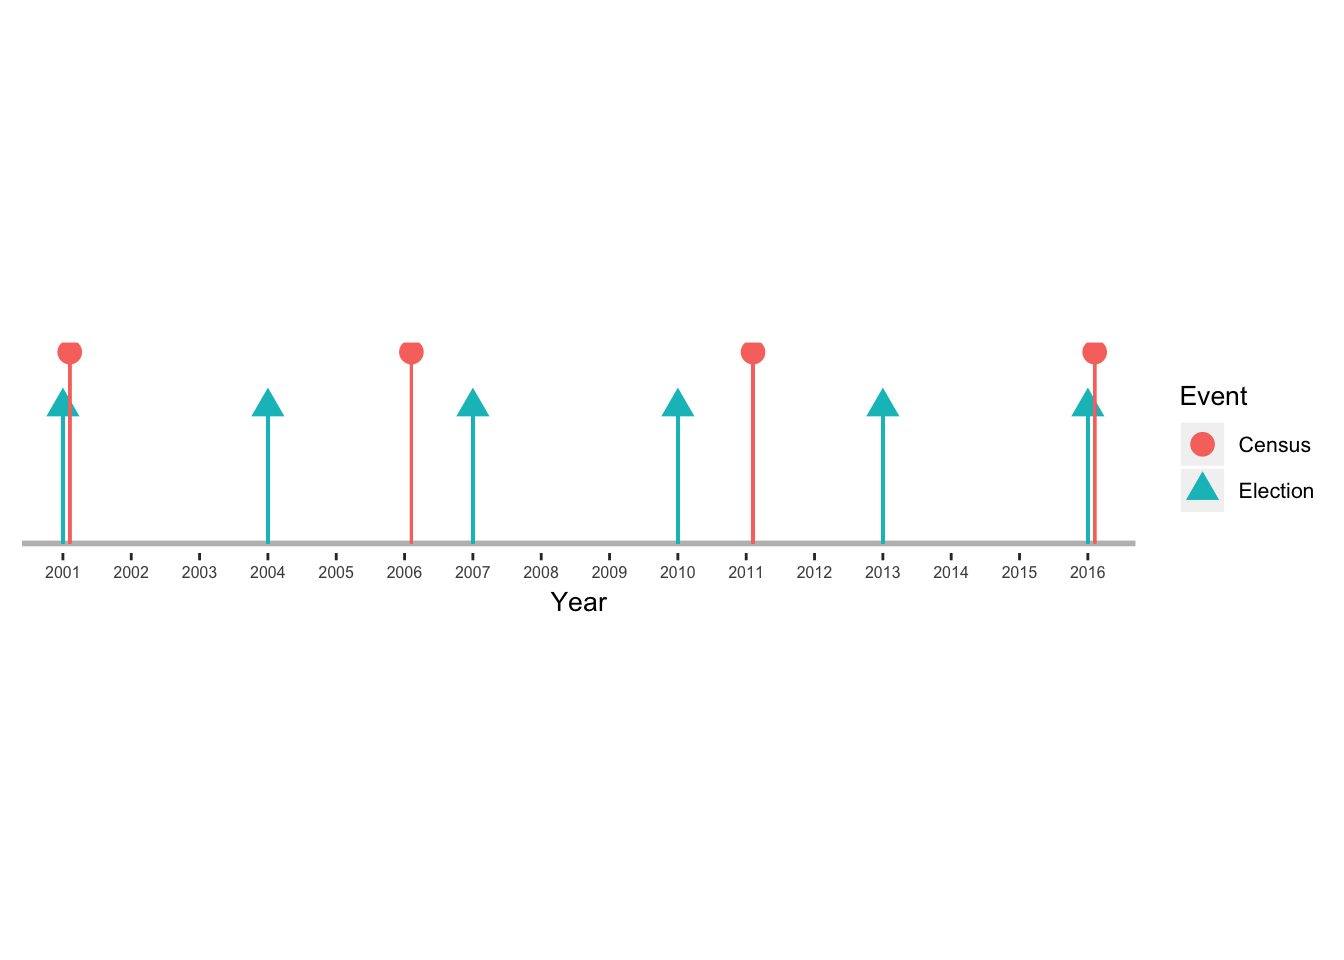
\includegraphics[width=0.9\linewidth]{anzjs_elections_files/figure-latex/timeline-1} 

}

\caption{Timeline of Australian elections and Censuses. They do not always occur in the same year.}\label{fig:timeline}
\end{figure}

\hypertarget{spatio-temporal-imputation}{%
\subsubsection*{Spatio-temporal imputation}\label{spatio-temporal-imputation}}
\addcontentsline{toc}{subsubsection}{Spatio-temporal imputation}

For each election, neighbouring Census information has to be combined in some way so that it represents the boundaries in place at the time of the election. This is done by taking the electoral boundaries and imputing the corresponding socio-demographic characteristics for each of the neighbouring Censuses, thereby addressing the spatial aspect. Next, to deal with the temporal component, characteristics at the time of the election are constructed using linear interpolation between the spatially imputed neighbouring Census variables.

The finest level of disaggregation available for Census data is the region classification called Statistical Area 1 (SA1). In 2016, Australia was divided into over 55,000 SA1s. Consider each of these SA1 regions as a source zone, \(s = 1,\dots,S\), for which socio-demographic information is available. For simplicity, let each source zone be wholly summarised by its centroid. A set of target zones, \(t = 1,\dots,T\), are defined as regions for which information is to be imputed --- these are the electoral boundaries for a particular election.

Take the example of the Melbourne Ports electorate from the 2013 federal election, illustrated in Figure \ref{fig:melbports13}. The purple region in this figure represents the target zone and the source zones are the centroid locations from the 2016 Census SA1 areas.

\begin{figure}[h]

{\centering \includegraphics[height=0.28\textheight]{anzjs_elections_files/figure-latex/melbports13-1} 

}

\caption{The electoral boundaries for Melbourne Ports (shown in purple) and surrounding electorates, with centroids for Statistical Area 1 regions from the 2016 Census overlaid. The centroids falling within the purple region are attributed to Melbourne Ports.}\label{fig:melbports13}
\end{figure}

Furthermore, let \(I_{s,t}\) be an indicator variable, for which \(I_{s,t} = 1\) if the centroid of source zone \(s\) falls within target zone \(t\), and \(0\) otherwise. Additionally, let the population of the source zone \(s\) be \(P_{s}\).

In order to calculate socio-demographic information for each of the target zones, a weighted average of source zones is taken using their populations as weights. Denote a given Census variable for the target zone by \(C_t\), and the same Census variable for the source zone as \(D_s\). Then, estimate \(C_t\) using
\[
  \hat{C}_t = \frac{\sum_{s=1}^{S}{I_{s,t}*D_s*P_s}}%
  {\sum_{s=1}^{S}{I_{s,t}*P_s}},
  \quad\text{for each $t=1,\dots,T$}.
\]

This concludes the spatial imputation of the socio-demographic characteristics for one target zone (a single electoral boundary), at the time of only one of the neighbouring Censuses. This process is repeated for all of the target zones, and then for the other neighbouring Census.

\enlargethispage*{0.5cm}

To account for temporal changes, linear interpolation is used between Census years to get the final estimate of a Census variable for the target zone in the election year. Let \(y_1\) be the year of the Census preceding an election, let \(y_2\) be the year of the election, and \(y_3\) be the year of the Census that follows. Add this year subscript to the Census variable estimate \(\hat{C}_t\), resulting in \(\hat{C}_{t,y}\). Linear interpolating between these Census years results an imputed value for the election year, given by
\[
  \hat{C}_{t,y_2} = \frac{y_3-y_2}{y_3-y_1} \hat{C}_{t,y_1} +
    \frac{y_2-y_1}{y_3-y_1} \hat{C}_{t,y_3}.
\]
Implicitly this assumes that population characteristics change in a linear manner over time.

Continuing with the example of Melbourne Ports in the 2013 election, the estimate for a given Census variable in 2016, \(\hat{C}_{\text{MelbPorts}, 2016}\) would be obtained by computing the weighted average of this variable amongst the SA1s within the purple region shown in Figure \ref{fig:melbports13}. This would be repeated with the 2011 Census SA1s to obtain \(\hat{C}_{\text{MelbPorts}, 2011}\), from which the final estimate is given by
\[
  \hat{C}_{\text{MelbPorts},2013}
    = \frac{3}{5} \hat{C}_{\text{MelbPorts},2011} + \frac{2}{5} \hat{C}_{\text{MelbPorts},2016}.
\]
This is done for each of the socio-demographic variables, and is repeated for each of the 149 remaining target zones corresponding with 2013 electorates.

\hypertarget{modelling}{%
\section{Modelling}\label{modelling}}

From this imputation process, electoral socio-demographic variables are available for each of the six elections and can be joined with their corresponding two-party preferred votes. Before choosing an appropriate model, two issues with the socio-demographic variables need to be addressed. First, variable scales change over the years, making it important to standardize variables. Second, many variables represent similar information and where appropriate, will be grouped together. To determine which variables should be grouped, principal component analysis (PCA) is used to guide the construction of specific factors. The intuition here is that PCA will identify which variables covary, from which intuitive groupings of variables can be chosen to combine into individual variables. Details are given in Section 3.2. After these steps, a model specification is chosen.

\hypertarget{standardizing-variables}{%
\subsection{Standardizing variables}\label{standardizing-variables}}

Many of the socio-demographic variables have changing scales over the years. For example, inflation-adjusted median rental prices increased across almost all electorates, with median rent of 225 dollars per week placing an electorate in the 90th percentile in 2001, but only the 45th percentile in 2016. In order for socio-demographic effects to be comparable across years, all explanatory variables are standardized to have mean zero and variance one within each election year. By standardizing, each variable is reported as a relative measure compared to all other electorates in the same year.

\hypertarget{creating-factors}{%
\subsection{Creating factors}\label{creating-factors}}

There are only \(N = 150\) observations (electorates) in each election and \(p = 50\) socio-demographic variables in each cross-section, with many variables representing similar information about an electorate. Any model that uses all variables would face problems with multi-collinearity and over-fitting, which would likely lead to erroneous conclusions regarding variable significance. To address this, a subset of variables that represent similar information are combined into a single variable, which will be referred to as a ``factor''.

A factor is created from a group of variables if there is an intuitive reason as to why these variables should represent similar information and if there is evidence to suggest that they covary. For example, a potential group would be variables relating to electoral incomes --- median family, household and personal incomes. To determine which variables covary, principal component analysis is used on a combined dataset of socio-demographic variables from all six elections\footnote{It is appropriate to compute principal components on a combined dataset of all six elections because when computed separately for each election, scree plots level off after four components and the loadings of the first four components are similar across the elections.}. The only variables exempted from the principal component analysis are the four variables representing age brackets (the proportion of the population aged 0--19 years old, 20--34 years old, 45--54 years old and 55 years plus), which are included in the model as separate variables.

Only the first four principal components from the combined dataset are considered, as the scree plot levels off after the fourth component. Variables that have a large loading in a particular component are deemed to covary, with a loading with magnitude greater than 0.15 being considered large. Each principal component is considered separately. If a subset of variables have large loadings (positive or negative) in a given component, and there is an intuitive reason as to why they should be grouped together, then this subset of variables will be combined to become a factor. Note that more than one factor can be deduced from a principal component (i.e.~multiple non-overlapping subsets of variables), and that any variables not included in a factor are not discarded.

Six factors are created using this approach. These are:
\texttt{Incomes} (median personal income, median household income, median family income);
\texttt{Unemployment} (unemployment rate, labour force participation rate);
\texttt{PropertyOwned} (proportion of dwellings that are owned, proportion of dwellings that are mortgages, proportion of dwellings that are rented, proportion of dwellings that classified as government housing);
\texttt{RentLoanPrice} (median rental payment amount, median loan repayment amount);
\texttt{FamHouseSize} (average household size, ratio of people to families, incidence of single person households, incidence of households containing a couple with kids, incidence of households containing a couple without kids); and
\texttt{Education} (high school completions, undergraduate and postgraduate degrees, proportion of employed people working as professionals, proportion of jobs in finance, proportion of workers who are labourers, proportion of workers who work as a tradesperson, diploma and certificate qualifications).

For each of these groupings, a factor is created by taking a weighted sum of the variables. The weightings are allocated on the basis of whether the variable had a positive or negative loading in the principal component from which the grouping was identified. Variables with a positive loading are allocated a weight of \(+1\) and those with negative loadings are allocated a weight of \(-1\). After computing these weighted sums, the factor is standardized to have mean zero and variance one, within each election.

The final predictor set contains \(p=32\) variables\footnote{The factor creation procedure reduces the variable set to \(p=33\), however one of the age brackets (\texttt{Pop\_55\_plus}) is not included as a variable to avoid multicollinearity, because the other three age brackets are included.} which are listed in Table \ref{tab:printmodels}.

\hypertarget{regression-incorporating-spatially-dependent-errors}{%
\subsection{Regression incorporating spatially dependent errors}\label{regression-incorporating-spatially-dependent-errors}}

An identical model specification is used for each of the six elections, with each election modelled separately. Separate models are preferred to a single model because of how frequently electoral boundaries change, noting that electorates with the same name across elections are not guaranteed to represent the same geographic region. Therefore any fixed or random effects models would be difficult to estimate without implementing consistent boundaries, which would require further imputation (of voting information). The separate models also allow the socio-demographic effects to be estimated separately for each election year, facilitating analysis of temporal changes in variable effects. This can be considered a special case of a longitudinal model where all coefficients are time-varying and heteroskedasticity is time-varying.

For each cross-section, let the response \(\bm{y}\) be the vector two-party preferred vote in favour of the Liberal party; for example, \(y_i = 70\) represents a 70\% preference for Liberal, 30\% for Labor, in electorate \(i\). Although \(y_i\) lies in the interval \((0,100)\), observed values are never close to 0 or 100 (minimum \(24.05 \%\) and maximum \(74.90 \%\)), so there is no need to formally impose the constraint of \(y_i \in [0,100]\). Furthermore, the responses are found to be spatially correlated in each election (Moran's I test, \(p \le 7\cdot10^{-15}\)). This is not surprising as electorates are aggregate spatial units, and hence the spatial structure of the data must be modelled appropriately.

The spatial error model \citep{Anselin88} is chosen because it captures spatial heterogeneity by incorporating a spatially structured random effect vector \citep{LeSage2009}. In this context, the random effect can be thought of as capturing the effect of any characteristics that neighbourhoods share that have not been addressed by the independent variables included in the model.

\begin{table}[!htbp]\vspace*{-0.4cm}\centering    \caption{Estimated spatial error model parameters (standard errors) for each of the six election years.\vspace*{-0.4cm}}    \label{tab:printmodels}  \fontsize{7}{8}\rm\tabcolsep=0.42cm \begin{tabular}{@{\extracolsep{1pt}}lrrrrrr} \\[-1.8ex]\hline  \hline \\[-1.8ex]  \\[-1.8ex] & \multicolumn{6}{c}{\vspace{-0.4cm}} \\   & 2001 & 2004 & 2007 & 2010 & 2013 & 2016 \\  \hline \\[-1.8ex]  $\rho$ & 0.53\rlap{$^{***}$} & 0.33\rlap{$^{**}$} & 0.21 & 0.17 & 0.27 & 0.39\rlap{$^{**}$}\\  & (0.15\rlap{)} & (0.16\rlap{)} & (0.18\rlap{)} & (0.17\rlap{)} & (0.17\rlap{)} & (0.17\rlap{)}\\  AusCitizen & $-$3.94\rlap{$^{*}$} & $-$1.39 & $-$2.18 & $-$1.28 & $-$3.89 & $-$2.66 \\    & (2.27\rlap{)} & (2.44\rlap{)} & (2.21\rlap{)} & (2.69\rlap{)} & (2.51\rlap{)} & (2.61\rlap{)} \\    Pop\_00\_19 & 0.49 & 2.66 & 9.39\rlap{$^{***}$} & 5.25 & 3.31 & 0.88 \\    & (2.54\rlap{)} & (3.91\rlap{)} & (3.63\rlap{)} & (3.64\rlap{)} & (2.91\rlap{)} & (2.62\rlap{)} \\    Pop\_20\_34 & $-$8.04\rlap{$^{***}$} & $-$7.72\rlap{$^{***}$} & $-$8.34\rlap{$^{***}$} & $-$11.68\rlap{$^{***}$} & $-$9.29\rlap{$^{***}$} & $-$9.21\rlap{$^{***}$} \\    & (1.80\rlap{)} & (2.21\rlap{)} & (2.18\rlap{)} & (2.90\rlap{)} & (2.62\rlap{)} & (2.37\rlap{)} \\    Pop\_35\_54 & $-$2.64\rlap{$^{***}$} & $-$2.78\rlap{$^{***}$} & $-$3.62\rlap{$^{***}$} & $-$3.13\rlap{$^{***}$} & $-$2.76\rlap{$^{**}$} & $-$2.13\rlap{$^{**}$} \\    & (0.84\rlap{)} & (0.89\rlap{)} & (0.83\rlap{)} & (1.10\rlap{)} & (1.11\rlap{)} & (1.06\rlap{)} \\    BornAsia & 3.58\rlap{$^{*}$} & $-$1.09 & 0.66 & $-$1.78 & $-$1.08 & $-$0.14 \\    & (2.09\rlap{)} & (2.52\rlap{)} & (1.99\rlap{)} & (2.74\rlap{)} & (2.54\rlap{)} & (2.17\rlap{)} \\    BornMidEast & $-$1.02 & $-$1.75 & $-$0.98 & $-$1.00 & $-$1.66 & $-$1.31 \\    & (1.00\rlap{)} & (1.17\rlap{)} & (1.09\rlap{)} & (1.33\rlap{)} & (1.23\rlap{)} & (1.11\rlap{)} \\    BornSEEuro & $-$1.63 & $-$3.17\rlap{$^{*}$} & $-$1.07 & $-$2.04 & $-$2.89\rlap{$^{***}$} & $-$2.53\rlap{$^{***}$} \\    & (1.37\rlap{)} & (1.68\rlap{)} & (1.06\rlap{)} & (1.29\rlap{)} & (1.11\rlap{)} & (0.97\rlap{)} \\    BornUK & 0.29 & 0.31 & 0.32 & 0.28 & $-$0.15 & $-$0.61 \\    & (1.02\rlap{)} & (1.04\rlap{)} & (0.87\rlap{)} & (1.06\rlap{)} & (0.99\rlap{)} & (0.99\rlap{)} \\    BornElsewhere & $-$4.13 & $-$1.51 & $-$1.03 & 2.45 & $-$4.21 & $-$2.17 \\    & (3.14\rlap{)} & (3.62\rlap{)} & (3.18\rlap{)} & (4.13\rlap{)} & (3.90\rlap{)} & (3.76\rlap{)} \\    Buddhism & $-$0.07 & 0.80 & 0.58 & $-$0.14 & $-$0.43 & $-$1.16 \\    & (1.31\rlap{)} & (1.54\rlap{)} & (1.39\rlap{)} & (1.66\rlap{)} & (1.60\rlap{)} & (1.58\rlap{)} \\    Christianity & $-$1.70 & $-$1.01 & $-$0.45 & 0.13 & 2.03 & 3.76\rlap{$^{**}$} \\    & (1.62\rlap{)} & (1.75\rlap{)} & (1.60\rlap{)} & (1.85\rlap{)} & (1.68\rlap{)} & (1.83\rlap{)} \\    CurrentlyStudying & $-$2.20\rlap{$^{*}$} & $-$0.01 & $-$0.14 & 1.35 & 0.32 & 0.22 \\    & (1.22\rlap{)} & (1.50\rlap{)} & (1.39\rlap{)} & (1.41\rlap{)} & (1.35\rlap{)} & (1.56\rlap{)} \\    DeFacto & $-$3.24 & $-$2.25 & $-$4.67\rlap{$^{**}$} & $-$7.75\rlap{$^{**}$} & $-$7.82\rlap{$^{**}$} & $-$10.39\rlap{$^{***}$} \\    & (2.07\rlap{)} & (2.62\rlap{)} & (2.27\rlap{)} & (3.09\rlap{)} & (3.08\rlap{)} & (3.15\rlap{)} \\    DiffAddress & 3.06\rlap{$^{***}$} & 2.75\rlap{$^{**}$} & 0.73 & 2.55 & 2.27 & 5.20\rlap{$^{***}$} \\    & (0.94\rlap{)} & (1.20\rlap{)} & (1.24\rlap{)} & (1.79\rlap{)} & (1.67\rlap{)} & (1.51\rlap{)} \\    Distributive & 1.60 & 1.89\rlap{$^{*}$} & 0.50 & 0.62 & 1.59 & 1.31 \\    & (1.06\rlap{)} & (1.14\rlap{)} & (0.99\rlap{)} & (1.27\rlap{)} & (1.20\rlap{)} & (1.18\rlap{)} \\    Education & $-$0.37 & $-$0.26 & $-$6.72\rlap{$^{**}$} & $-$7.31\rlap{$^{*}$} & $-$7.31\rlap{$^{**}$} & $-$8.55\rlap{$^{**}$} \\    & (2.35\rlap{)} & (3.34\rlap{)} & (3.00\rlap{)} & (3.90\rlap{)} & (3.63\rlap{)} & (3.37\rlap{)} \\    Extractive & 3.74\rlap{$^{***}$} & 4.96\rlap{$^{***}$} & 4.64\rlap{$^{***}$} & 6.46\rlap{$^{***}$} & 5.97\rlap{$^{***}$} & 6.38\rlap{$^{***}$} \\    & (1.43\rlap{)} & (1.47\rlap{)} & (1.20\rlap{)} & (1.45\rlap{)} & (1.35\rlap{)} & (1.38\rlap{)} \\    FamHouseSize & 1.94 & $-$2.55 & $-$6.47\rlap{$^{**}$} & $-$3.84 & $-$3.12 & $-$2.00 \\    & (2.61\rlap{)} & (3.66\rlap{)} & (3.28\rlap{)} & (3.87\rlap{)} & (3.52\rlap{)} & (3.06\rlap{)} \\    Incomes & 4.36\rlap{$^{***}$} & 2.42 & 5.52\rlap{$^{**}$} & 5.63\rlap{$^{*}$} & 8.02\rlap{$^{***}$} & 12.70\rlap{$^{***}$} \\    & (1.69\rlap{)} & (3.00\rlap{)} & (2.42\rlap{)} & (3.15\rlap{)} & (2.78\rlap{)} & (2.64\rlap{)} \\    Indigenous & 1.26 & 1.96 & 2.41 & 2.38 & 0.46 & $-$0.22 \\    & (1.61\rlap{)} & (1.89\rlap{)} & (1.59\rlap{)} & (2.00\rlap{)} & (1.88\rlap{)} & (1.90\rlap{)} \\    Islam & $-$0.75 & $-$0.91 & $-$0.60 & $-$2.01 & $-$0.88 & $-$1.09 \\    & (1.14\rlap{)} & (1.28\rlap{)} & (1.14\rlap{)} & (1.41\rlap{)} & (1.26\rlap{)} & (1.30\rlap{)} \\    Judaism & 1.32 & 0.93 & 1.47 & 0.28 & 1.35 & 1.15 \\    & (1.01\rlap{)} & (1.08\rlap{)} & (0.92\rlap{)} & (1.10\rlap{)} & (1.02\rlap{)} & (0.97\rlap{)} \\    ManagerAdmin & 2.62\rlap{$^{***}$} & 4.67\rlap{$^{***}$} & 7.47\rlap{$^{***}$} & 7.05\rlap{$^{***}$} & 5.93\rlap{$^{***}$} & 5.64\rlap{$^{***}$} \\    & (0.67\rlap{)} & (1.06\rlap{)} & (0.95\rlap{)} & (1.16\rlap{)} & (1.06\rlap{)} & (0.97\rlap{)} \\    Married & $-$3.93 & $-$2.72 & $-$9.35\rlap{$^{***}$} & $-$10.12\rlap{$^{***}$} & $-$7.91\rlap{$^{**}$} & $-$9.47\rlap{$^{**}$} \\    & (2.51\rlap{)} & (3.56\rlap{)} & (3.12\rlap{)} & (3.55\rlap{)} & (3.57\rlap{)} & (3.85\rlap{)} \\    NoReligion & $-$0.73 & 0.04 & 1.32 & 0.37 & 1.41 & 2.94 \\    & (1.50\rlap{)} & (1.65\rlap{)} & (1.51\rlap{)} & (1.75\rlap{)} & (1.74\rlap{)} & (2.03\rlap{)} \\    OneParentHouse & $-$4.77\rlap{$^{***}$} & $-$3.23 & $-$6.55\rlap{$^{***}$} & $-$7.03\rlap{$^{***}$} & $-$5.32\rlap{$^{***}$} & $-$4.94\rlap{$^{**}$} \\    & (1.49\rlap{)} & (1.99\rlap{)} & (1.81\rlap{)} & (2.04\rlap{)} & (1.97\rlap{)} & (2.03\rlap{)} \\    OtherLanguage & $-$1.02 & 6.88 & 6.21 & 7.80 & 10.13\rlap{$^{**}$} & 9.98\rlap{$^{**}$} \\    & (3.00\rlap{)} & (4.93\rlap{)} & (3.97\rlap{)} & (5.25\rlap{)} & (5.09\rlap{)} & (4.26\rlap{)} \\    PropertyOwned & $-$2.01 & $-$0.30 & 0.74 & $-$1.92 & $-$1.05 & 0.73 \\    & (1.35\rlap{)} & (1.49\rlap{)} & (1.36\rlap{)} & (1.74\rlap{)} & (1.67\rlap{)} & (1.48\rlap{)} \\    RentLoanPrice & $-$2.17 & 0.37 & 1.23 & 3.08 & 1.36 & $-$2.04 \\    & (1.46\rlap{)} & (1.93\rlap{)} & (1.76\rlap{)} & (2.23\rlap{)} & (2.20\rlap{)} & (2.07\rlap{)} \\    SocialServ & 3.31\rlap{$^{***}$} & 2.85\rlap{$^{**}$} & 3.46\rlap{$^{***}$} & 3.72\rlap{$^{**}$} & 2.98\rlap{$^{**}$} & 4.04\rlap{$^{***}$} \\    & (1.27\rlap{)} & (1.40\rlap{)} & (1.17\rlap{)} & (1.46\rlap{)} & (1.28\rlap{)} & (1.15\rlap{)} \\    Transformative & 2.30 & 4.71\rlap{$^{***}$} & 4.58\rlap{$^{***}$} & 4.55\rlap{$^{**}$} & 3.63\rlap{$^{**}$} & 4.05\rlap{$^{***}$} \\    & (1.48\rlap{)} & (1.77\rlap{)} & (1.51\rlap{)} & (1.87\rlap{)} & (1.67\rlap{)} & (1.47\rlap{)} \\    Unemployment & $-$3.39\rlap{$^{**}$} & $-$3.47\rlap{$^{**}$} & $-$0.40 & $-$0.68 & 0.81 & 1.93 \\    & (1.37\rlap{)} & (1.69\rlap{)} & (1.45\rlap{)} & (1.80\rlap{)} & (1.47\rlap{)} & (1.32\rlap{)} \\    Constant & 50.80\rlap{$^{***}$} & 52.63\rlap{$^{***}$} & 47.31\rlap{$^{***}$} & 49.92\rlap{$^{***}$} & 53.52\rlap{$^{***}$} & 50.46\rlap{$^{***}$} \\    & (0.76\rlap{)} & (0.59\rlap{)} & (0.44\rlap{)} & (0.52\rlap{)} & (0.54\rlap{)} & (0.64\rlap{)} \\  Residual Standard Error (GLS\rlap{)} & 4.34 & 4.82 & 4.32 & 5.30 & 4.82 & 4.76\\  \hline \\[-1.8ex]  Observations & 150 & 150 & 150 & 150 & 150 & 150 \\  \hline  \hline \\[-1.8ex]  & \multicolumn{6}{r}{$^{*}$p$<$0.1; $^{**}$p$<$0.05; $^{***}$p$<$0.01} \\ \end{tabular}  \end{table}

Spatial weights are calculated in accordance with the assumption that an electorate is equally correlated with any electorate that shares a part of its boundary. Let \(\rho\) be the spatial autoregressive coefficient, \(\bm{v}\) be a spherical error term, \(\bm{W}\) be a matrix of spatial weights (containing information about the neighbouring regions), \(\bm{X}\) be a matrix of socio-demographic covariates, \(\bm{\beta}\) be a vector of regression coefficients and \(\bm{a}\) be a spatially structured random effect vector.
\[
  \bm{y} = \bm{X} \bm{\beta} + \bm{a},
\]
and
\[
  \bm{a} = \rho \bm{W} \bm{a} + \bm{v},
\]
where \(\bm{v} \sim N(\bm{0}, \sigma^2 \bm{I_n})\), and hence
\[
  \bm{y} = \bm{X} \bm{\beta} + (\bm{I}_n-\rho \bm{W})^{-1}\bm{v}.
\]
Estimation of the above spatial error model is undertaken using feasible generalized least squares.

Table \ref{tab:printmodels} details the estimated model coefficients and their estimated standard errors, for each of the six elections. An interpretation of these estimated values is provided in the next section.

\hypertarget{results}{%
\section{Results}\label{results}}

\hypertarget{spatial-autoregressive-parameter}{%
\subsection{Spatial autoregressive parameter}\label{spatial-autoregressive-parameter}}

The spatial autoregressive coefficient \(\rho\) is positive and significant in the 2001, 2004 and 2016 elections (Figure \ref{fig:rhovis}). In these three elections, there is evidence to suggest that neighbours share some influential characteristics outside the explanatory variables, which affect the two-party preferred vote. Conversely, in the other three elections, the spatial effect weakens to become insignificant (although still positive).

\begin{figure}[h]

{\centering 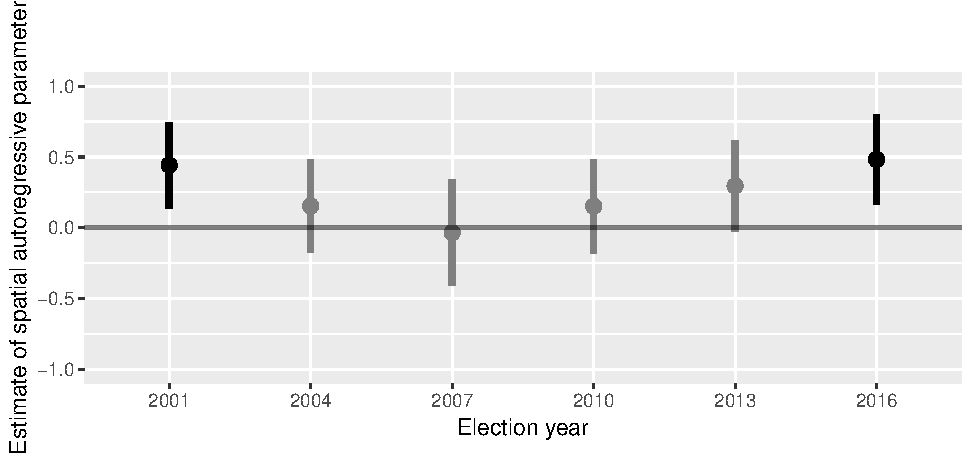
\includegraphics[height=0.2\textheight,]{anzjs_elections_files/figure-latex/rhovis-1} 

}

\caption{Estimates of the spatial autoregressive parameter for each of the six elections, reported with their individual 95\% confidence intervals. In 2001, 2004 and 2016 there is a significant spatial component.}\label{fig:rhovis}
\end{figure}

\hypertarget{country-wide-trend}{%
\subsection{Country-wide trend}\label{country-wide-trend}}

\begin{figure}[h]

{\centering 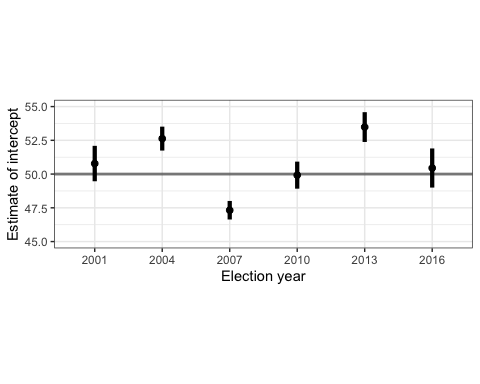
\includegraphics[height=0.2\textheight,]{anzjs_elections_files/figure-latex/plotintercept-1} 

}

\caption{Estimated intercept for each election, which represents the two-party preferred vote for an electorate with mean characteristics.}\label{fig:plotintercept}
\end{figure}

Since all socio-demographics have been standardized to have a mean of zero and a variance of one, the intercept in each model can be interpreted as the estimated two-party preferred vote for an electorate with mean characteristics\footnote{Mean of all variables aside from Judaism, Indigenous, Islam and Buddhism, where it assumes the mean of the log value.}. Figure \ref{fig:plotintercept} shows that the baseline of party preference has varied over the elections, with the biggest swing occurring in the 2007 election where the mean electorate shifted more than five percentage points in favour of the Labor party.

\hypertarget{influential-socio-demographics}{%
\subsection{Influential socio-demographics}\label{influential-socio-demographics}}



\begin{figure}[h]

{\centering 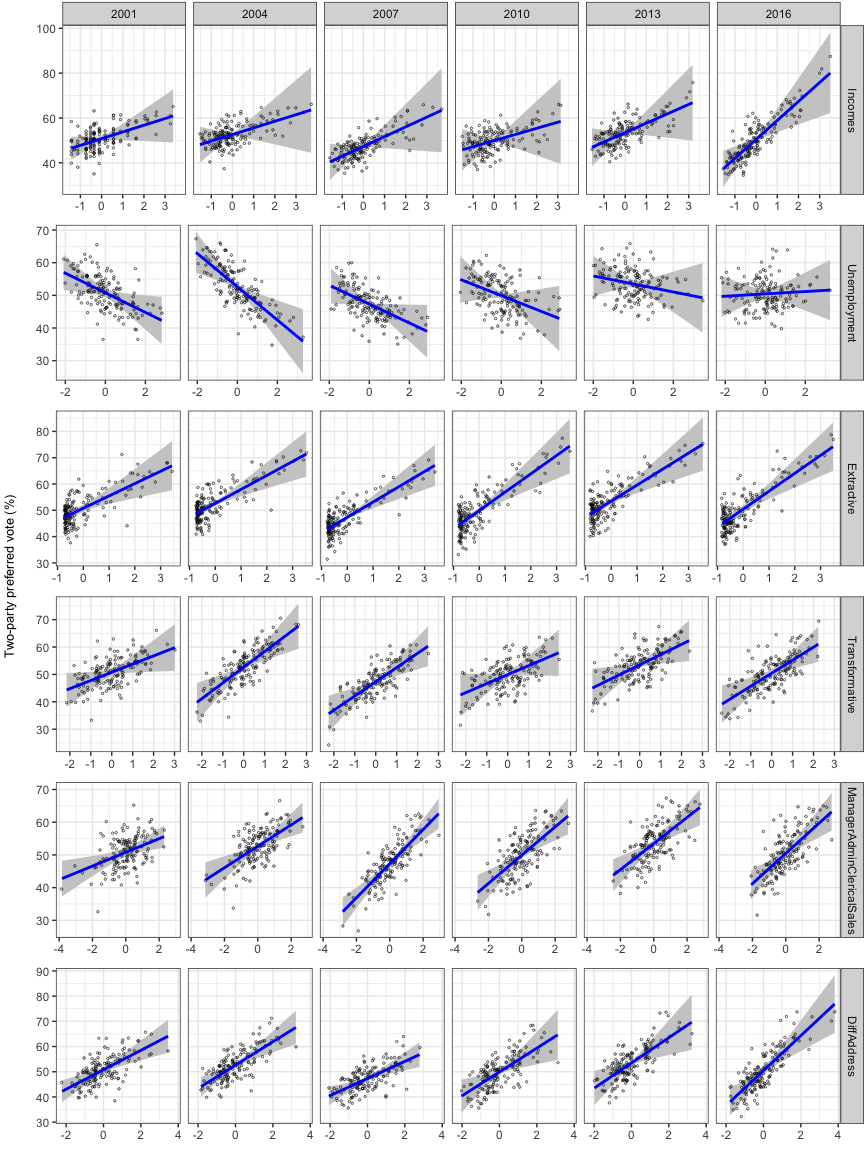
\includegraphics{anzjs_elections_files/figure-latex/partresplot1-1} 

}

\caption{Partial residual plots by election year for a selection of predictors. Linear model with 95\% confidence bands overlaid. Most predictors have a positive relationship: the larger the value the more likely the electorate preferences Liberal. The relationship is relatively robust over time, with the exception of \texttt{DiffAddress}, \texttt{Incomes}, \texttt{OtherLanguageHome} and \texttt{Pop\_00\_19}.}\label{fig:partresplot1}
\end{figure}



\begin{figure}[h]

{\centering 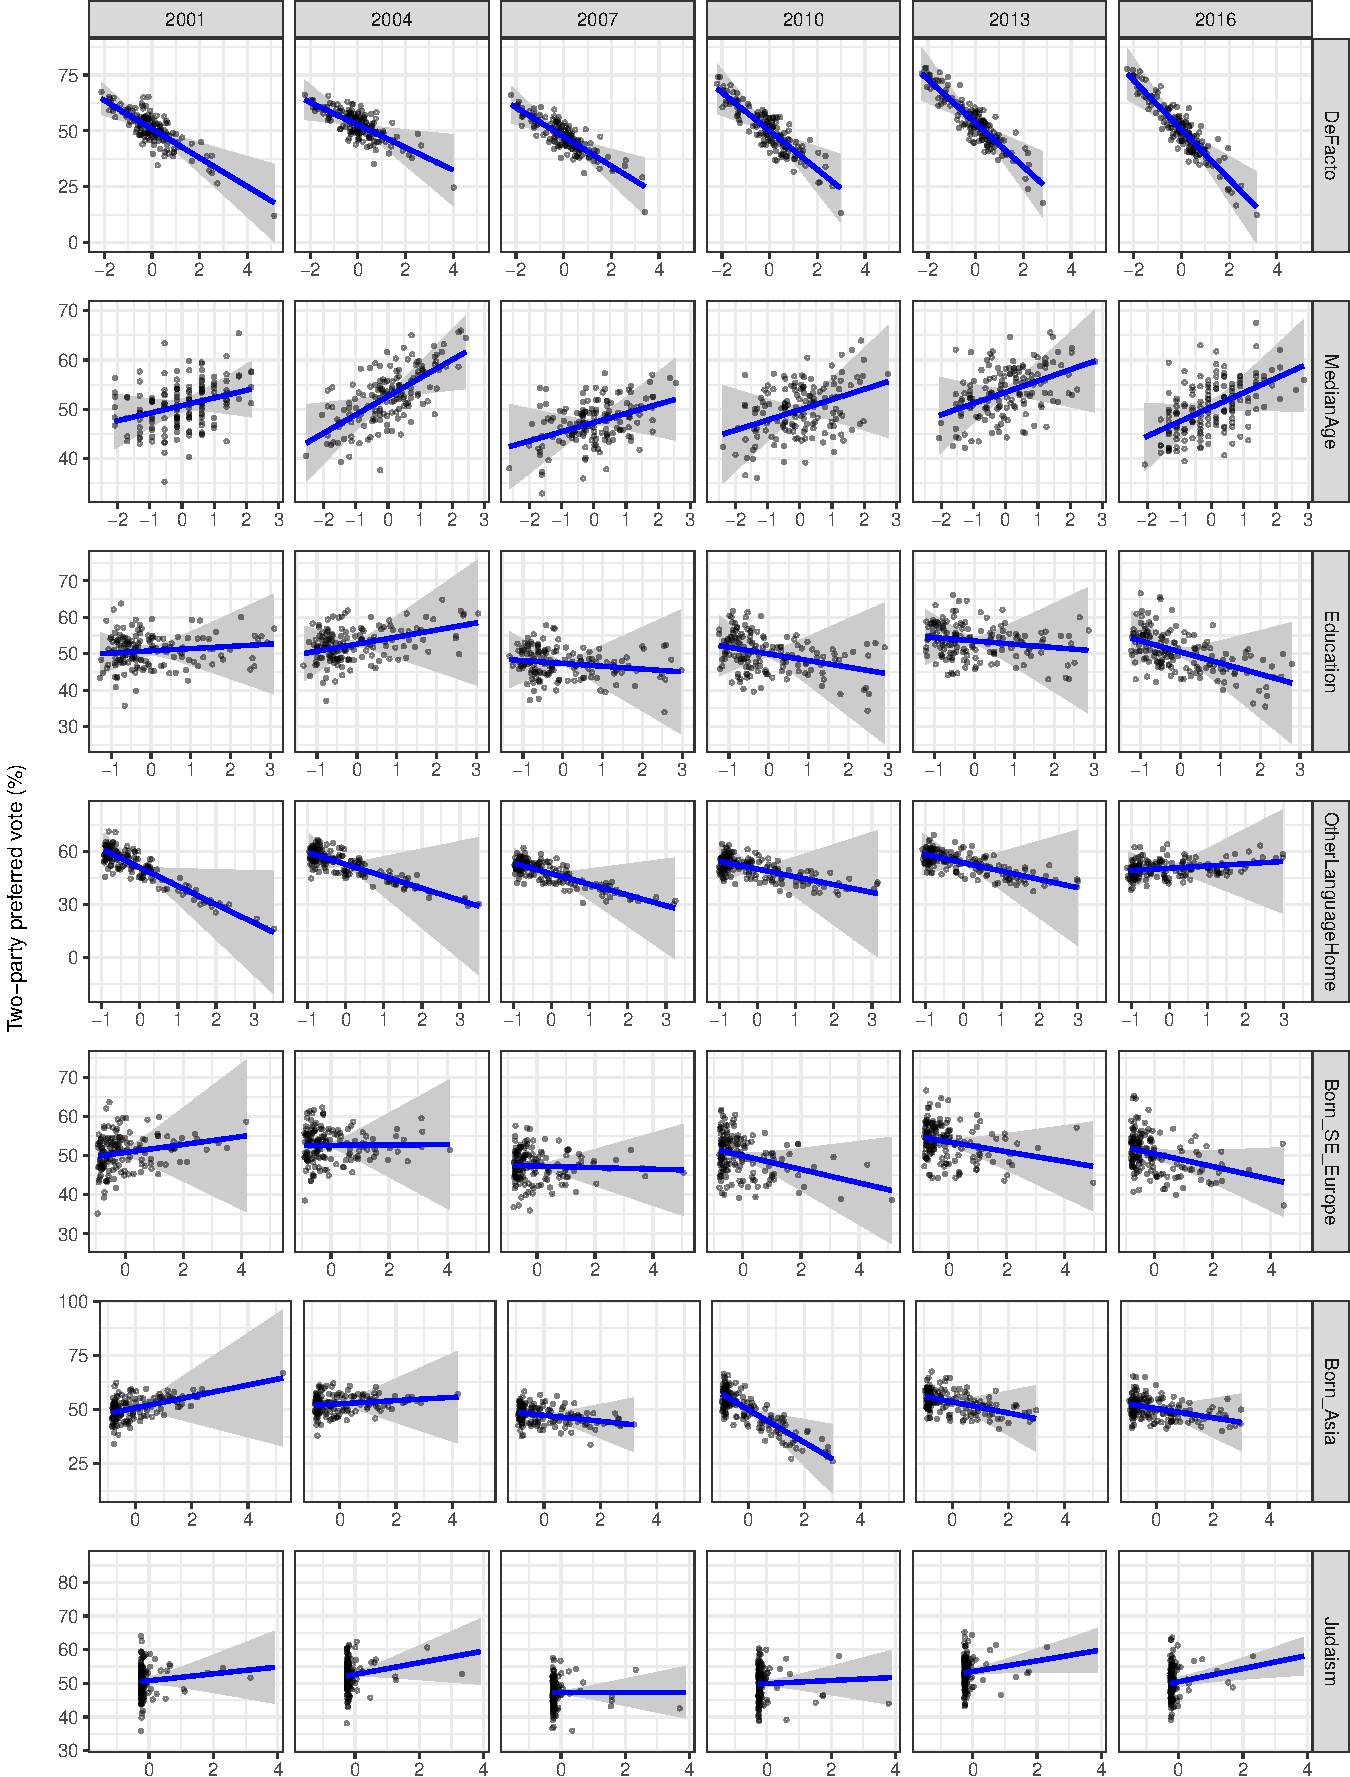
\includegraphics{anzjs_elections_files/figure-latex/partresplot2-1} 

}

\caption{Partial residual plots by election year for a selection of predictors. Linear model with 95\% confidence bands overlaid. Several predictors have a negative relationship: with larger values indicating the electorate more likely preferences Labor. Most relationships are relatively stable over elections, except \texttt{Unemployment} and \texttt{Education}."}\label{fig:partresplot2}
\end{figure}

To investigate the socio-demographics that have a strong effect on the two-party preferred vote, partial residual plots are used and shown in Figures \ref{fig:partresplot1} and \ref{fig:partresplot2}. Partial residuals, for a given variable, are the residuals from the fitted model with the estimated effect of that variable added to it. These plots show the direction, size and significance of an estimated effect, as well as any deviations from linearity. In each plot, the slope of the prediction line matches the estimated coefficient and the shaded region represents a 95\% confidence band. Plots are computed using the method in \citet{visreg}. If a horizontal line can be drawn through the confidence band, then the effect is insignificant. The estimated intercept is also added to the partial residuals for interpretability. Plots for each election are faceted to compare the effects over time in Figures \ref{fig:partresplot1} and \ref{fig:partresplot2}. Only socio-demographics that have a significant effect in at least two elections are displayed in Figures \ref{fig:partresplot1} and \ref{fig:partresplot2}.

\hypertarget{industry-and-type-of-work}{%
\subsubsection*{Industry and type of work}\label{industry-and-type-of-work}}
\addcontentsline{toc}{subsubsection}{Industry and type of work}

Electorates with higher proportions of workers in mining, gas, water, agriculture, waste and electricity (grouped as \texttt{Extractive} industries) are consistently linked with higher support for the Liberal party, with the magnitude of this effect slightly increasing over the years (see row 1 in Figure \ref{fig:partresplot1}). This is unsurprising, as the Liberal party has close ties with these traditional energy industries, and typically present policies to reduce taxation on energy production. Furthermore, electorates with more workers in construction or manufacturing industries (\texttt{Transformative}) are also more likely to support the Liberal party (see row 3 in Figure \ref{fig:partresplot1}), from 2004 onwards.

Similarly, the proportion of workers in managerial, administrative, clerical and sales roles (\texttt{ManagerAdmin}), is also a significant predictor of two-party preference vote across all six elections, with a higher proportion of people working these jobs increasing Liberal support.

Of these job related variables, the most surprising effect is that associated with the proportion of workers in education, healthcare, social work, community and arts (\texttt{SocialServ}). Typically the Labor party has more generous funding schemes affecting these areas of work, so one might expect \texttt{SocialServ} to have a negative effect on two-party preference. However, in every election this effect is found to be positive and significant.

\hypertarget{income-and-unemployment}{%
\subsubsection*{Income and unemployment}\label{income-and-unemployment}}
\addcontentsline{toc}{subsubsection}{Income and unemployment}

Typically the Labor party campaigns on more progressive policies, which often include tax reform that adversely affects higher income earners, and more generous social assistance programs. Perhaps it is due to these policies that higher income electorates appear more likely to support the Liberal party, as the \texttt{Incomes} factor has a positive effect on Liberal preference (see row 6 in Figure \ref{fig:partresplot1}). This effect is significant in every election aside from 2004 and 2010. \texttt{Unemployment} however, is not as influential. In 2001 and 2004, electorates with higher unemployment align with Labor, but over time this shifts towards support for the Liberal party, culminating in a positive (insignificant) effect in 2016.

\hypertarget{age}{%
\subsubsection*{Age}\label{age}}
\addcontentsline{toc}{subsubsection}{Age}

The older Australian population is often believed to be more conservative, and the left leaning political parties (including Labor) typically have a stronger appeal to younger people. This effect is indeed observed across the six elections, with populations between 20 and 34 years of age (\texttt{Pop\_20\_34}) being very strongly aligned with Labor preference (bottom row in Figure \ref{fig:partresplot2}). Larger populations of 35 to 54 year olds (\texttt{Pop\_35\_54}) are also associated with Labor, but the magnitude of this effect is far smaller. Populations under 20 years of age is only significant in 2007, where \texttt{Pop\_00\_19} increased Liberal support.

\hypertarget{education}{%
\subsubsection*{Education}\label{education}}
\addcontentsline{toc}{subsubsection}{Education}

Since 2007, electorates with higher education levels are associated with supporting the Labor party, with this effect being significant in 2007, 2013 and 2016 and only marginally insignificant in 2010. In the elections before 2007, education has a negligible effect (see row 3 in Figure \ref{fig:partresplot2}). Additionally, student populations (\texttt{CurrentlyStudying}) do not affect electoral party preference in any election (not shown).

\hypertarget{diversity}{%
\subsubsection*{Diversity}\label{diversity}}
\addcontentsline{toc}{subsubsection}{Diversity}

Larger migrant populations from Asia, the Middle East, South-Eastern Europe, the United Kingdom and elsewhere, are either associated with Labor support, or have no effect. Of these areas, only South-Eastern European populations significantly affect party preference, with larger populations associating with Labor in 2013 and 2016 (row 2, Figure \ref{fig:partresplot2}). Speaking other languages (aside from English) however, appears to have a far stronger effect, as observed through the \texttt{OtherLanguage} variable. Electorates with more diverse speech are associated with higher support for the Liberal party from 2004 onwards, with this effect being significant in 2013 and 2016 (see row 7, Figure \ref{fig:partresplot1}). Furthermore, none of the variables relating to religious beliefs aside from Christianity have a material effect in any election (this includes the Buddhist, Muslim, Jewish, non-religious and Indigenous Australian populations). The association between Christian populations (\texttt{Christianity}) and the Liberal party steadily increases over the years, becoming positive and significant in 2016.

\hypertarget{households}{%
\subsubsection*{Households}\label{households}}
\addcontentsline{toc}{subsubsection}{Households}

In 2001, 2004 and 2016, higher proportions of people that have recently (in the past five years) moved house (\texttt{DiffAddress}) increased electoral support for the Liberal party (see row 5 in Figure \ref{fig:partresplot1}). This is somewhat surprising as one might expect house ownership and rental prices to be linked to two-party preference, rather than household mobility (\texttt{PropertyOwned} and \texttt{RentLoan} are not significant in any election).

Higher proportions of single parent households are associated with Labor support in all elections (albeit insignificant in 2004, see row 6 in Figure \ref{fig:partresplot2}), whereas the electoral family and household sizes (via the \texttt{FamHouseSize} variable) do not appear to be associated with either party.

\hypertarget{relationships}{%
\subsubsection*{Relationships}\label{relationships}}
\addcontentsline{toc}{subsubsection}{Relationships}

From 2007 onwards, both marriages (\texttt{Married}) and de facto relationships (\texttt{DeFacto}) are found to be strong predictors of the two-party preferred vote in favour of the Labor party. In 2001 and 2004 neither of these variables are significant (see rows 4 and 5 in Figure \ref{fig:partresplot2}).

\hypertarget{a-closer-look-at-the-residuals}{%
\subsection{A closer look at the residuals}\label{a-closer-look-at-the-residuals}}

\hypertarget{residuals-by-state}{%
\subsubsection*{Residuals by state}\label{residuals-by-state}}
\addcontentsline{toc}{subsubsection}{Residuals by state}

It is often hypothesized that states have a systematic bias towards one of the two major parties. Boxplots of residuals grouped by state (Figure \ref{fig:resstate}) show that the data reflects this to only a limited extent. Tasmania and the Australian Capital Territory appear to have a bias towards Labor, whereas the South Australia and the Northern Territory tend towards voting Liberal. However, there are relatively few electorates in each of these states (five, two, eleven and two respectively), so this apparent result may be due to incumbent effects rather than an actual state-specific bias.

\begin{figure}[h]

{\centering 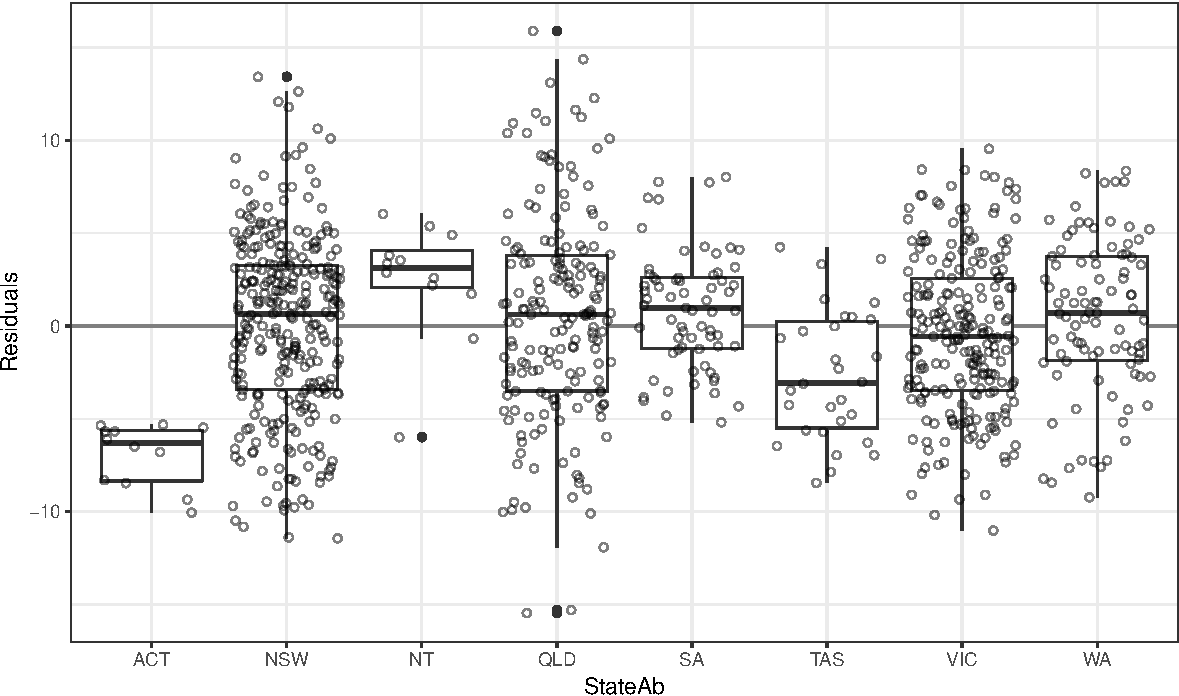
\includegraphics[width=0.7\linewidth,]{anzjs_elections_files/figure-latex/resstate-1} 

}

\caption{Boxplot of residuals by state with jittered points. States ordered by median residual. A state-specific bias present only in the smaller states appears to have not been captured by the model.}\label{fig:resstate}
\end{figure}

\hypertarget{residuals-by-party-incumbency}{%
\subsubsection*{Residuals by party incumbency}\label{residuals-by-party-incumbency}}
\addcontentsline{toc}{subsubsection}{Residuals by party incumbency}

The incumbent party appears to have a distinct advantage at the next election. The boxplots in Figure \ref{fig:resincumbent} show that if either of the Labor or Liberal parties won the seat at the previous election, the electorate is likely to vote in their favour, over and above any socio-demographic effects --- this effect has not been captured by the model.

\begin{figure}[h]

{\centering \includegraphics[width=0.7\linewidth,]{anzjs_elections_files/figure-latex/resincumbent-1} 

}

\caption{Boxplot of residuals for incumbent and non-incumbent parties each year. An incumbent advantage is evident and has not been captured by the model.}\label{fig:resincumbent}
\end{figure}

\hypertarget{robustness}{%
\subsection{Robustness}\label{robustness}}

\hypertarget{multicollinearity}{%
\subsubsection*{Multicollinearity}\label{multicollinearity}}
\addcontentsline{toc}{subsubsection}{Multicollinearity}

Three robustness checks are conducted to confirm model stability. First, a model for each election is re-estimated using only the variables that are found to be significant in at least one of the six elections. The estimated coefficients of the variables in the re-estimated models all fall within their respective 95\% confidence intervals from the full models. The second check involves the ten largest pairwise correlations. For each pair, a model for each election is re-estimated omitting one of the two variables. It is found that for each of these pairs, the estimated effect of the remaining variable in the reduced model lies within the 95\% confidence interval from the full model. The final check is a visual exploration of different variable projections using a tour \citep{tourr} for each election. No definitive signs of multicollinearity are observed, and as expected (given the nature of spatial data), there is some clumping of electorates for certain projections.

\hypertarget{influential-and-outlier-electorates}{%
\subsubsection*{Influential and outlier electorates}\label{influential-and-outlier-electorates}}
\addcontentsline{toc}{subsubsection}{Influential and outlier electorates}

Based on the distribution of the Cook's distance values and the distribution of hat values, a Cook's distance greater than \(0.1\) is considered to be influential, and a hat value greater than \(0.5\) is considered to have high leverage. Electorates fitting these criteria are flagged and investigated to examine the characteristics driving these values.

The electorate of Sydney (NSW) has a large Cook's distance and high leverage from 2001 to 2007, due to its diverse population (languages, birthplace and religion), high density of young adults (20 to 34 years old), high number of defacto relationships, high income, high household mobility and small amount of workers in extractive and transformative jobs. It has remained a strong supporter of the Labor party and the extent of this support is underpredicted by the model, making it an outlier. Nearby in metropolitan NSW, the electorate of Wentworth is found to be an outlier in the 2013 and 2016 elections. Although historically Liberal, its two-party vote jumped by over 10 percentage points in 2010 without experiencing any notable changes in its socio-demographic makeup --- implying that this may be the direct effect of its Liberal member, Malcolm Turnbull, becoming the leader of the Liberal party. In the elections since, the model underpredicts Wentworth's Liberal support.

Lingiari, an electorate taking up almost all of the Northern Territory, has consistently high leverage (all years) and is an outlier in all but the 2013 election due to its large Indigenous population, low rates of property ownership and few workers in management or administrative jobs. Fowler (NSW) has a diverse population with a high proportion of migrants, many Buddhists and Muslims, as well as a high proportion of single parent households. These characteristics explain its high leverage in 2001, 2004, 2010 and 2013, and its strong Labor support makes it influential in 2001, 2004 and 2010. Other electorates with large Cook's distance are Canberra (ACT) and Durack (WA) in 2013, and Solomon (NT) in 2016.

All of the electorates examined are not unduly influential in the model and therefore no action is required.

\hypertarget{conclusion}{%
\section{Conclusion}\label{conclusion}}

This paper explores the effects of electoral socio-demographic characteristics on the two-party preferred vote in the 2001--2016 elections, using information from the corresponding Australian federal elections and Censuses. As a Census does not always occur in the same year as an election, Census data for the 2004--2013 elections are generated by employing a method of spatio-temporal imputation. This imputes electoral socio-demographics for the electoral boundaries in place at the time of the election --- an approach that is distinctly different from previous work on modelling election outcomes, where Census and election data are typically joined without addressing their temporal differences. Before estimating a model, these socio-demographic variables are standardized (to adjust for changing variable scales) and subsets of variables (representing similar information) are combined into factors, resulting in a reduced predictor set. A spatial error model is then estimated for each election, accounting for the inherent spatial structure of the data.

Across the past six elections, most of the socio-demographics that drive the electoral two-party preferred vote are found to remain steady, whilst a few (typically weaker) effects vary over time. Industry and type of work are particularly influential. Energy-related and manufacturing/construction jobs, as well as administrative roles and jobs in education and social services are strongly linked with the Liberal party in all elections. Incomes have a similarly consistent effect, with higher income areas supporting Liberal. Higher levels of unemployment shift from weak association with Labor to a significant Liberal effect over the years, and higher education levels are associated with Labor from 2007 (although marginally insignificant in 2010). Electorates with large populations 20 to 34 years are strongly associated with Labor, whilst the 35 to 54 year old bracket also increases Labor support, but to a lesser extent. It is also found that birthplace diversity slightly favours Labor, relationships (both marriages and de facto relationships) align with Labor preference from 2010 onwards, and the influence of Christian populations has trended towards Liberal support whilst other religions have negligible effects. Family and household sizes have minimal influence, although electorates with more single parent households are linked with Labor support. Furthermore, the spatial effects are found to be positive in all elections and significant in 2001, 2004 and 2016, meaning that other characteristics that neighbours have in common (outside of the variables in the model) appear to be influential in those years.

The findings in this paper complement the existing literature by modelling temporal trends, which as far as the authors are aware, has not been done previously for Australian elections using a regression framework. It is also the first study to model any Australian election since 2010 using Census information.

Additionally, a key contribution of this research is the wrangling of the raw data and imputed data sets for the 2004, 2007, 2010 and 2013 elections, which have been contributed to the \texttt{eechidna} \texttt{R} package --- providing a rich, accessible data resource for any future Australian electoral analysis.

\hypertarget{acknowledgements}{%
\section{Acknowledgements}\label{acknowledgements}}

This paper was produced using \texttt{RMarkdown} \citep{rmarkdown} and \texttt{knitr} \citep{knitr}. All corresponding code for this paper can be found in the github repository \href{https://github.com/jforbes14/eechidna-paper}{github.com/jforbes14/eechidna-paper}, and the data used is available in the \texttt{eechidna} package \citep{eechidna}. All raw data was obtained from the Australian Electoral Commission, the Australian Bureau of Statistics and the Australian Government.

The authors would like to sincerely thank the editor and associate editor of the Australian \& New Zealand Journal of Statistics and the two anonymous reviewers for providing helpful comments and suggestions on earlier drafts of this manuscript. Additionally, the authors would like to thank Anthony Ebert, Heike Hofmann, Thomas Lumley, Ben Marwick, Carson Sievert, Mingzhu Sun, Dilini Talagala, Nicholas Tierney, Nathaniel Tomasetti, Earo Wang and Fang Zhou, all of whom have contributed to the \texttt{eechidna} package.

\hypertarget{software}{%
\section{Software}\label{software}}

All election and Census datasets, along with electoral maps and more, are available in the \texttt{eechidna} (Exploring Election and Census Highly Informative Data Nationally for Australia) \texttt{R} package, which can be downloaded from CRAN. The \texttt{eechidna} package makes it easy to look at the data from the Australian Federal elections and Censuses that occurred between 2001 and 2016. This study contributed a large revision to the \texttt{eechidna} package, which included the addition of election and Census data for 2001--2010, voting outcomes for polling booths and imputed Census data for election years. For more details on using \texttt{eechidna}, please see the articles (vignettes) on the github page \href{https://ropenscilabs.github.io/eechidna/}{ropenscilabs.github.io/eechidna/}.

\renewcommand\refname{References}
\bibliography{references.bib}


\end{document}
